\section{A: Preamble}

\begin{frame}%[fragile]
\frametitle{About the Course}
%
These course notes were originally based on:\\[1em]
{\bf C By Dissection (3rd edition)}\\
{\it Al Kelley and Ira Pohl}\\[1em]

because I liked arrays being taught late(r).
I've since changed my mind a little \& have re-jigged the notes quite heavily for this year.
\end{frame}

\begin{frame}%[fragile]
\frametitle{Resources}
\begin{itemize}[<+->]
\item Free : \url{https://en.wikibooks.org/wiki/C_Programming}
\item A list of more : \url{https://www.linuxlinks.com/excellent-free-books-learn-c/}
\item Whatever you use, make sure it's {\bf ANSI C} or {\bf C99} that's being taught, not something else e.g.\ C11 or C++.
\item If you fall in love with C and  know you're going to use it for the rest of your life, the reference `bible' is K\&R 2nd edition.
It's not a textbook for those new to programming, though.
\begin{figure}[h]
\centerline{

\includegraphics[scale=0.25]{../Figs/9780131103627.jpg}
}
\end{figure}
\end{itemize}
\end{frame}

\begin{frame}%[fragile]
\frametitle{Computer Science Ethos}
\begin{itemize}[<+->]
\item Talk to your friends, ask for help, work together.
\item Never pass off another persons work as your own.
\item Do not pass work to others - either on paper or
electronically - even after the submission deadline.
\item If someone takes your code and submits it, we need to investigate where it originated - all students involved
will be part of this.
\item Don't place your code on publicly accessible sites e.g. github - other students may have extensions etc.
\end{itemize}
\end{frame}

\begin{frame}%[fragile]
\frametitle{History of C}

\begin{columns}
\begin{column}{0.5\textwidth}

\begin{figure}[h]
\centerline{
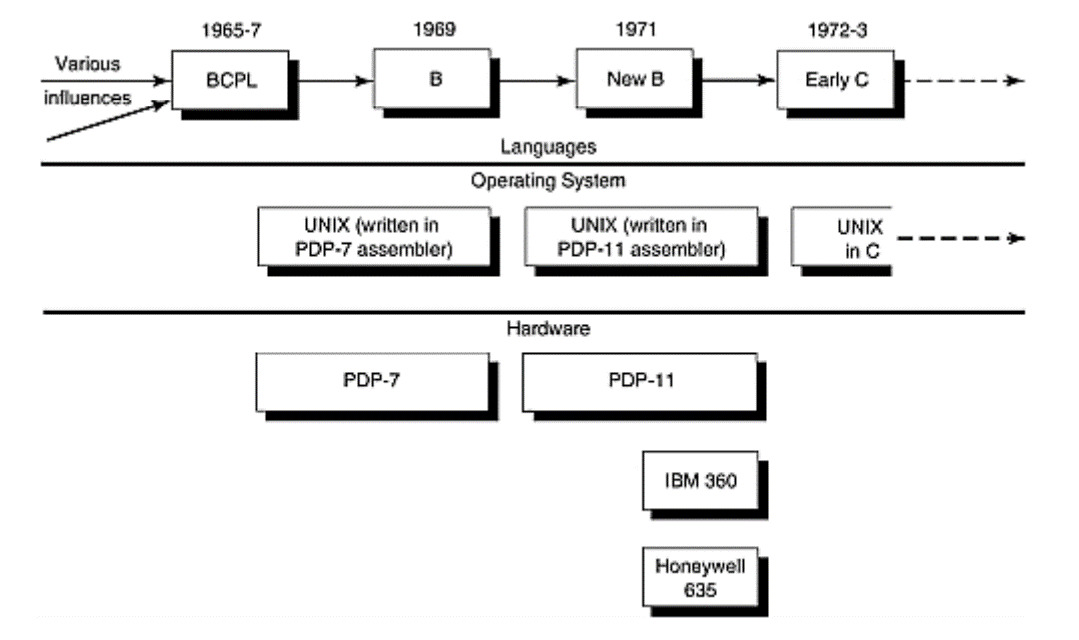
\includegraphics[width=1.0\textwidth]{../Figs/evolvec.jpg}
}\centerline{
{\tiny From {\bf Deep C Secrets} by {\it Peter Van Der Linden}}
}
\end{figure}
\end{column}

\begin{column}{0.5\textwidth}
\begin{itemize}[<+->]
\item BCPL - Martin Richards
\item B - Ken Thomson 1970
\item Both of above are {\em typeless}.
\item C - Dennis Ritchie 1972 designed for\\(\& implemented on) a UNIX system.
\item K\&R C (Kernighan and Ritchie) 1978
\item ANSI C
\item C99 (COMSM1201)
\item C++ - Object Oriented Programming (OOP)
\item Java (Subset of C++, WWW enabled).
\end{itemize}
\end{column}
\end{columns}
\end{frame}

\begin{frame}%[fragile]
\frametitle{Why C ?}

\begin{columns}

\begin{column}{0.5\textwidth}
\begin{figure}[h]
\centerline{
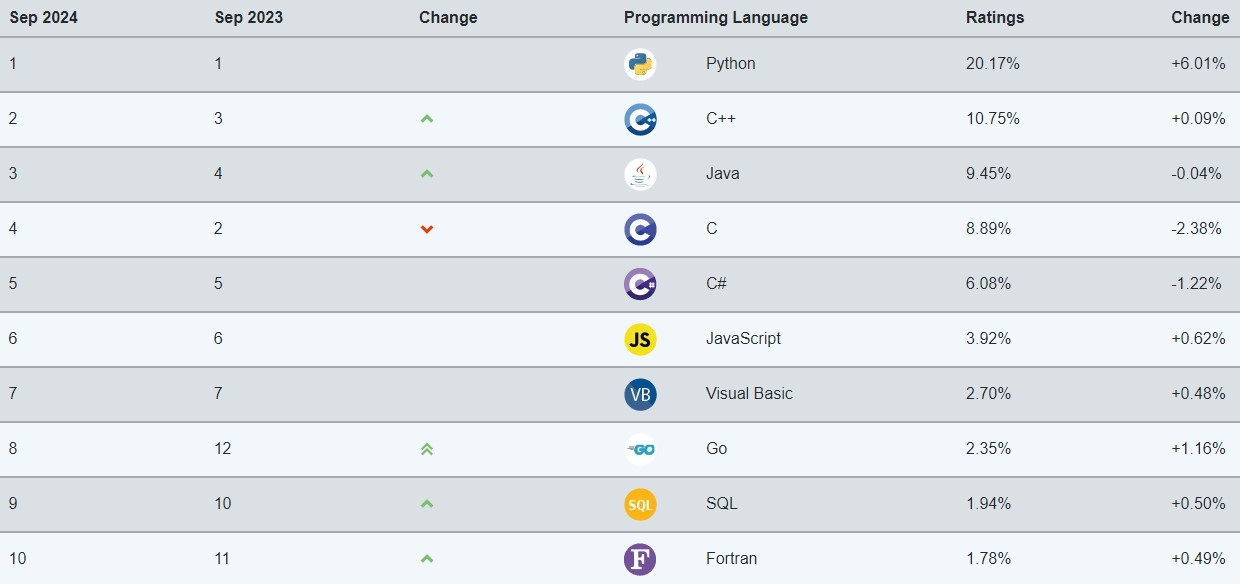
\includegraphics[width=1.0\textwidth]{../Figs/tiobe.jpg}
}
\centerline{
{\tiny \url{https://www.tiobe.com/tiobe-index/}}
}
\end{figure}
\end{column}

\begin{column}{0.5\textwidth}
\begin{itemize}[<+->]
\item One of the most commonly used programming languages
according to {\tt tiobe.com}
\item Low-level (c.f. Java)
\item Doesn't hide nitty-gritty
\item Fast ?
\item Large parts common to Java
\end{itemize}
\end{column}

\end{columns}
\end{frame}

\begin{frame}%[fragile]
\frametitle{Programming and Software Engineering}
\begin{itemize}[<+->]
\item Was traditionally Lectured 2(or 3) hours a week for weeks 1-12
\item In the blended world, I'll post the equivalent online, broken
into manageable chunks
\item Programming (C), data structures, algorithms - searching, sorting, string processing, trees etc.
\end{itemize}
\end{frame}

\begin{frame}%[fragile]
\frametitle{Assessment}
\begin{itemize}[<+->]
\item Weekly (unmarked) exercises that, if completed, should ensure you are able to pass the unit.
\item Approximately three/four assignments and one lab test.
\item One major project due in early TB2 (35\%).
\item Hard to gauge timings, so don't make any plans in advance -
I'll change it if we're going too fast.
\end{itemize}
\end{frame}


\begin{frame}%[fragile]
\frametitle{Help with Computers}
\begin{itemize}[<+->]
\item Any problems with the computers e.g. installing the correct S/W, accessing lab machines: \url{http://www.bris.ac.uk/it-services/}.
\item They are also the people to see about passwords etc.
\item This page also links to the rather useful Laptop \& Mobile Clinic.
\end{itemize}
\end{frame}

\begin{frame}%[fragile]
\frametitle{Help with the Unit}
\begin{itemize}[<+->]
\item Further information is available via the Blackboard site.
\item Help will mainly be via myself giving `live' Q\&A session, the associated MS Teams group and the corresponding Forum.
\item You will often work in a peer group (approx $15$ people).
\item There will be a group of Teaching Assistants to help each of these groups.
\item TAs are not allowed to write pieces of code for you,
nor undertake detailed bug-fixing of your program.
\end{itemize}
\end{frame}
